\let\negmedspace\undefined
\let\negthickspace\undefined
\documentclass[journal]{IEEEtran}
\usepackage[a5paper, margin=10mm, onecolumn]{geometry}
%\usepackage{lmodern} % Ensure lmodern is loaded for pdflatex
\usepackage{tfrupee} % Include tfrupee package

\setlength{\headheight}{1cm} % Set the height of the header box
\setlength{\headsep}{0mm}     % Set the distance between the header box and the top of the text

\usepackage{gvv-book}
\usepackage{gvv}
\usepackage{cite}
\usepackage{amsmath,amssymb,amsfonts,amsthm}
\usepackage{algorithmic}
\usepackage{graphicx}
\usepackage{textcomp}
\usepackage{xcolor}
\usepackage{txfonts}
\usepackage{listings}
\usepackage{enumitem}
\usepackage{mathtools}
\usepackage{gensymb}
\usepackage{comment}
\usepackage[breaklinks=true]{hyperref}
\usepackage{tkz-euclide} 
\usepackage{listings}
\def\inputGnumericTable{}                                 
\usepackage[latin1]{inputenc}                                
\usepackage{color}                                            
\usepackage{array}                                            
\usepackage{longtable}                                       
\usepackage{calc}                                             
\usepackage{multirow}                                         
\usepackage{hhline}                                           
\usepackage{ifthen}                                           
\usepackage{lscape}
\begin{document}

\bibliographystyle{IEEEtran}
\vspace{3cm}

\title{4.8.15}
\author{AI25BTECH11019 - MENAVATH SAI SANJANA}
{\let\newpage\relax\maketitle}

\renewcommand{\thefigure}{\theenumi}
\renewcommand{\thetable}{\theenumi}
\setlength{\intextsep}{10pt} % Space between text and floats

\numberwithin{equation}{enumi}
\numberwithin{figure}{enumi}
\renewcommand{\thetable}{\theenumi}

\textbf{Question}:\\
A line $l$ passes through point $(-1,3,-2)$ and is perpendicular to both the lines  
\begin{align}
\frac{x-1}{1} = \frac{y-1}{2} = \frac{z+1}{3}, \quad
\frac{x+2}{-3} = \frac{y}{2} = \frac{z}{5}.
\end{align}
Find the vector equation of the line $l$ and its distance from the origin.
\\
\bigskip
\textbf{Solution: }

Let the direction vector of the required line be
\begin{align}  
\vec{d} = \myvec{a\\b\\c}.
\end{align}  

Since the line is perpendicular to the two given lines, the direction vector satisfies
\begin{align}  
\vec{d}_1^\top \vec{d} &= 0 \quad \Rightarrow \quad 1\cdot a + 2\cdot b + 3\cdot c = 0,\\  
\vec{d}_2^\top \vec{d} &= 0 \quad \Rightarrow \quad -3\cdot a + 2\cdot b + 5\cdot c = 0.
\end{align}  

Solve the system:  
\begin{align}  
8b + 14c &= 0 \;\;\Rightarrow\;\; b = -\frac{7}{4}c,\\  
a + 2b + 3c &= 0 \;\;\Rightarrow\;\; a = \frac{1}{2}c.
\end{align}  

Choosing $c=4$ to get integer values:  
\begin{align}  
\vec{d} = \myvec{2\\-7\\4}.
\end{align}  

Vector equation of the line through $P=(-1,3,-2)$:  
\begin{align}  
\vec{r} = \myvec{-1\\3\\-2} + t\,\myvec{2\\-7\\4}, \quad t \in \mathbb{R}.
\end{align}  

Distance from origin:  
\begin{align}  
t &= -\frac{\vec{P}\cdot\vec{d}}{\vec{d}\cdot\vec{d}} 
= -\frac{(-1)(2) + 3(-7) + (-2)(4)}{2^2 + (-7)^2 + 4^2} 
= \frac{31}{69},\\  
\vec{Q} &= \vec{P} + t\vec{d} = \myvec{-\tfrac{7}{69}\\\\ -\tfrac{10}{69}\\\\ -\tfrac{14}{69}},\\  
D &= \|\vec{Q}\| = \sqrt{\tfrac{345}{69^2}} = \sqrt{\tfrac{5}{69}}.
\end{align}  

\vspace{1cm}

\noindent\textbf{Conclusion:}  
The required line is  
\begin{align}
\vec{r} = \myvec{-1\\3\\-2} + t\,\myvec{2\\-7\\4}, \quad t \in \mathbb{R},
\end{align}  
and its distance from the origin is  
\begin{align}
D = \sqrt{\tfrac{5}{69}}.
\end{align}

\begin{figure}[ht!]
    \centering
    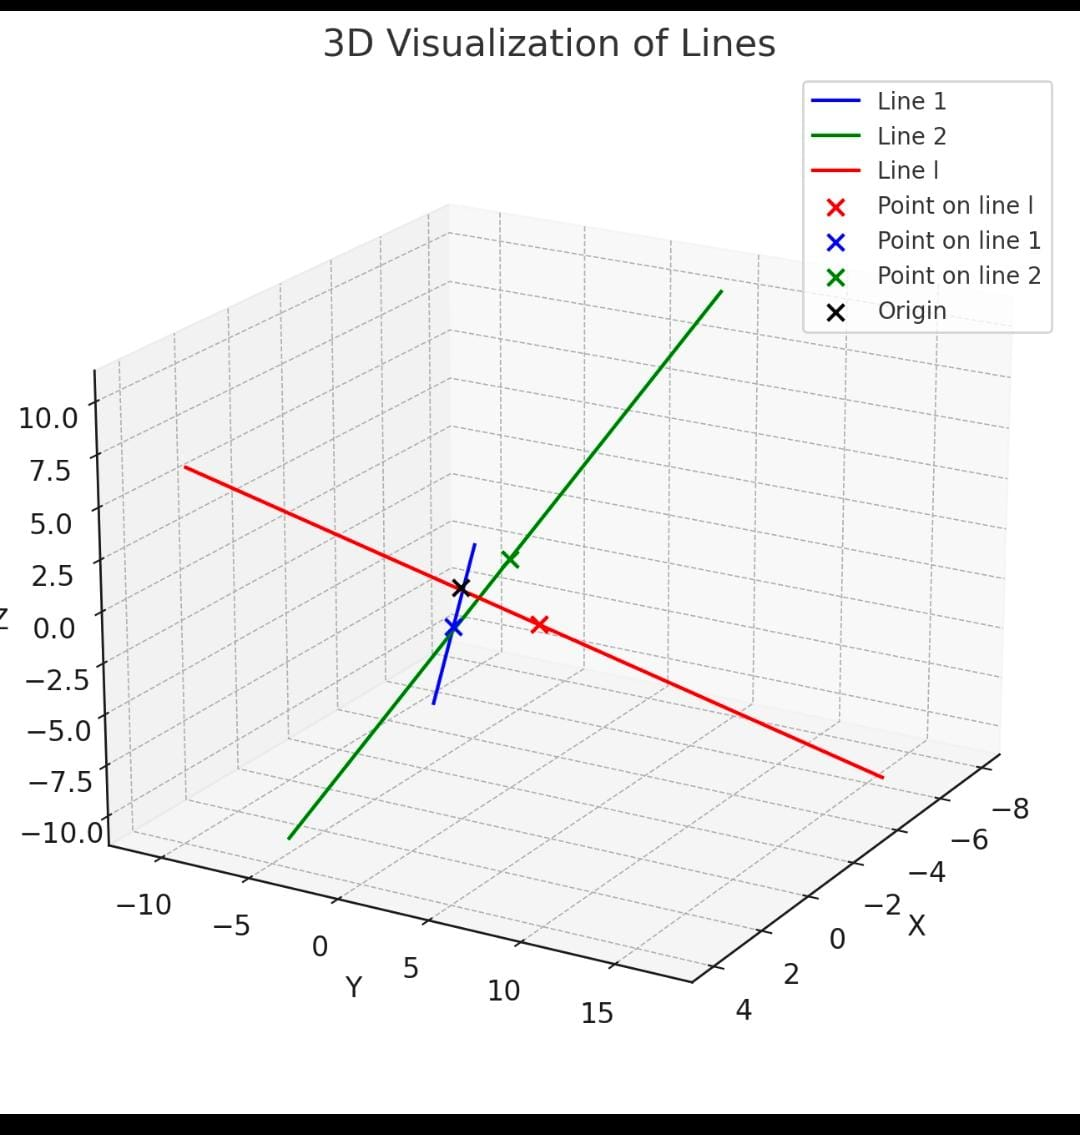
\includegraphics[width=0.8\textwidth]{figs/matgeo-4.8.15.jpeg}
    \caption{}
    \label{fig:3.3.4}
\end{figure}

\end{document}

